% "{'classe':(''),'chapitre':'','type':(''),'titre':'', 'source':' ','comp':(None),'corrige':True}"
%%%% Paramétrage du TD %%%%
\def\xxactivite{TD 02 \ifprof-- Corrigé \else \fi }
\def\xxauteur{\textsl{Xavier Pessoles}}
%\fancyfoot[C]{\rule{12cm}{.5pt}}
%\renewcommand{\footrulewidth}{0.2pt}
%\fancyfoot[C]{\footnotesize{\bfseries \thepage}}
%\fancyfoot[L]{ 
%\begin{minipage}[c]{.4\linewidth}
%\noindent\footnotesize{{\xxauteur}}
%\end{minipage}}


\def\xxnumchapitre{Chapitre 5 \vspace{.2cm}}
\def\xxchapitre{\hspace{.12cm} Rapidité des systèmes}

\def\xxcompetences{%
\textsl{%
\textbf{Savoirs et compétences :}\\
\vspace{-.4cm}
\begin{itemize}[label=\ding{112},font=\color{ocre}] 
\item C2-03 : Déterminer les performances d'un système asservi.
\end{itemize}
}}


\def\xxfigures{
\includegraphics[width=.4\linewidth]{fig_01}
}%figues de la page de garde

\def\xxtitreexo{Base TC200 Tecdron}
\def\xxsourceexo{\hspace{.2cm} \footnotesize{Centrale Supelect TSI 2021}}

\input{\repRel/Style/pagegarde_TD}

\setlength{\columnseprule}{.1pt}

\pagestyle{fancy}
\thispagestyle{plain}


\vspace{4.5cm}

\def\columnseprulecolor{\color{bleuxp}}
\setlength{\columnseprule}{0.4pt} 
%%%%%%%%%%%%%%%%%%%%%




\ifprof
\else
\begin{multicols}{2}
\fi


\setcounter{numques}{0}
\subsection*{Mise en situation}

Dans l’industrie, il est désormais possible d’associer des tâches robotisées et des tâches manuelles. Après l’essor
des robots collaboratifs, Tecdron, entreprise Française basée à La Rochelle, propose une base mobile nommée
TC200, capable de recevoir différents types de bras robotisés -- dont des bras collaboratifs -- mais aussi de
se déplacer de manière autonome dans un environnement industriel complexe composé de robots et d’humains.

Les figures ci-dessous donnent la structure du robot étudié. 

\begin{center}
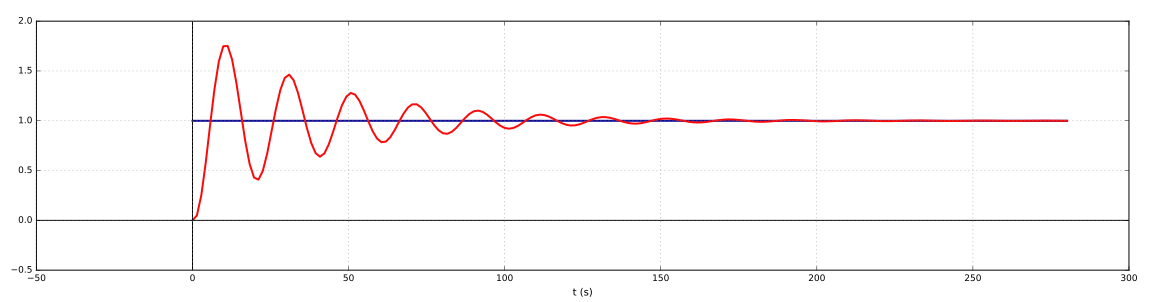
\includegraphics[width=\linewidth]{fig_02}

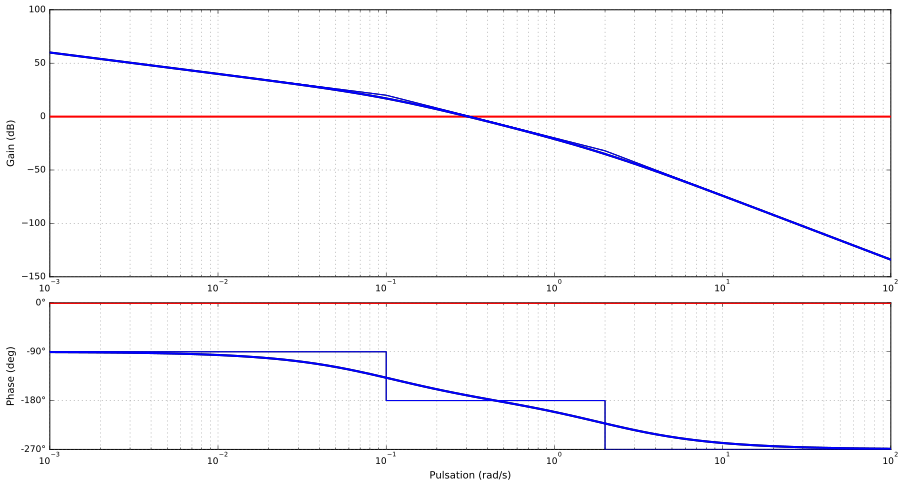
\includegraphics[width=\linewidth]{fig_03}
%\textit{}
\end{center}


\subsection*{Validation de l'asservissement du moteur}
\begin{obj}
Valider l’asservissement de vitesse mis en place pour que la base TC200 se déplace suivant la trajectoire
de consigne souhaitée.

Vérifier les exigences de la boucle de vitesse en termes de stabilité, précision et rapidité.
\end{obj}



\begin{center}
\includegraphics[width=\linewidth]{fig_04}
%\textit{}
\end{center}

La boucle de courant étant supposée parfaite, le schéma bloc de la figure 19 correspond à l’asservissement de
vitesse d’une des motorisations. Le modèle est considéré pour le moment non perturbé, c’est-à-dire $C_f(p)=0$.

\begin{center}
\includegraphics[width=\linewidth]{fig_05}
%\textit{}
\end{center}


\begin{center}
\includegraphics[width=\linewidth]{fig_06}
%\textit{}
\end{center}

\question{Déterminer la fonction de transfert en boucle fermée $\indice{H}{BF}(p)=\dfrac{\Omega_m(p)}{\Omega_{mc}(p)}$ pour $C_f(p)=0$.}
\ifprof
\begin{corrige}
\end{corrige}
\else
\fi

\question{Justifier que cet asservissement est stable et donner la valeur de la marge de phase.}
\ifprof
\begin{corrige}
\end{corrige}
\else
\fi


\question{Déterminer la condition sur $K_2$ afin de satisfaire l’exigence de rapidité.}
\ifprof
\begin{corrige}
\end{corrige}
\else
\fi


\question{Calculer l’erreur relative en régime permanent $\mu_{v \infty}$ pour une consigne de vitesse en échelon de valeur $\omega_{mc0}$.}
\ifprof
\begin{corrige}
\end{corrige}
\else
\fi

On donne les diagrammes de Bode de la FTBO.

\begin{center}
\includegraphics[width=\linewidth]{fig_07}
%\textit{}
\end{center}


\question{Identifier la valeur de $K_2$ qui a été réellement choisie par le constructeur.}
\ifprof
\begin{corrige}
\end{corrige}
\else
\fi

\question{À partir de cette valeur, calculer l’erreur en vitesse en régime permanent $\Delta \omega_{\infty}$ pour une consigne de vitesse en rampe de pente $a$ et valider le critère de précision des exigences.}
\ifprof
\begin{corrige}
\end{corrige}
\else
\fi





%\subsection*{Éléments de correction}
%\begin{enumerate}
%\item ...
%\item $\left(Mp^2+\mu p + k \right)\Delta Z(p) = S\Delta p (p)-\Delta F(p)$ et $\Delta Q(p)=S p \Delta Z(p) + \left( \varphi + \dfrac{V}{2b} p \right) \Delta P(p)$.
%\item ...
%\item $\Delta q = K\Delta U\sqrt{p_a - P_0} - \dfrac{KU_0}{2\sqrt{p_a - P_0}}\Delta p + \text{termes néglig.}$.
%\item ...
%\item ...
%\item $K_a = k_c$.
%\item $\text{FTBO}(p)=\dfrac{ABC(p)GE}{1+GDB+GE}$ et $\text{FTBF}(p)=\dfrac{\text{FTBO}(p)}{1+\text{FTBO}(p)}$.
%\item ...
%\item ...
%\item ...
%\item $\omega_0=\SI{83,6}{rad.s^{-1}}$ et $\xi=0,21$, $\omega_3 = \SI{0,75}{rad.s^{-1}}$.
%\item ...
%\item ...
%\end{enumerate}


\ifprof
\else
\end{multicols}
\fi





